\chapter{Algoritmo de Shor}
El algoritmo de Shor es un AC de factorización de enteros. Dado un entero $N=p \times q$, donde $p$ y $q$ son primos, el algoritmo de Shor encuentra $p$ y $q$ en $O((\log(N))^3)$ pasos. El algoritmo clásico más eficiente para factorizar enteros es la cibra general del cuerpo de números y funciona con una complejidad heurística de $O(e^{(\sqrt[3]{\frac{64}{9}}+o(1))(\ln(N))^{\frac{1}{3}}(\ln(\ln(N)))^{\frac{2}{3}}})$. Por su capacidad de factorizar números semiprimos, el algoritmo de Shor es capaz de violar el cifrado RSA y el protocolo Diffie-Hellman de intercambio de llaves, sobre los cuáles se basa virtualmente toda la criptografía actual.

El algoritmo de Shor requiere de dos algoritmos cuánticos preliminares: La estimación de fase y la estimación de orden. El algoritmo de estimación de fase permite encontrar la fase $\phi$ del autovalor $e^i \phi$ asociado a algún autoestado $\ket{u}$ de un operador unitario U. El algoritmo de estimación de orden se basa en la estimación de fase para hallar el orden $r>0$ tal que $a^r \equiv 1 \mod m$.

\section{Transformada cuántica de Fourier}

Una de las transformadas integrales cuánticas más importantes es la tranformada cuántica de Fourier. Sea $\omega_n$ la n-ésima raíz primitiva de la unidad:

\begin{equation}
    \omega_n = e^{2\pi i/N}
\end{equation}

Donde $N = 2^n$. El número complejo $\omega_n$ define el kernel K como:

\begin{equation}
    K(x,y) = \frac{1}{\sqrt{N}} \omega_n^{x y}
\end{equation}

La transformada integral discreta con el kernel K,

\begin{equation}
    \tilde{f}(y) = \frac{1}{\sqrt{N}} \sum\limits_x \omega^{-x y} f(x)
\end{equation}

se llama la transformada discreta de Fourier (DFT).

El kernel K es unitario ya que:

\begin{multline}
    (K K^\dagger)(x,y) = \bra{x} K K^\dagger \ket{y}
    = \bra{x} K \sum\limits_z \ketbra{z}{z} K^\dagger \ket{y} \\
    = \sum\limits_z K(x,z) K^\dagger(z,y) 
    = \frac{1}{N} \sum\limits_z \omega^{-x z} \omega^{y z} 
    = \frac{1}{N} \sum\limits_z \omega^{- (z-y) z} 
    = \delta_{x y}
\end{multline}

La transformada integral cuántica definida con este kernel se llama transformada cuántica de Fourier.

El kernel para $n = 1$ es:

\begin{equation}
    K_1 = \frac{1}{\sqrt{2}}
    \begin{pmatrix}
        1 & 1 \\
        1 & e^{2\pi i/2}
    \end{pmatrix} =
    \frac{1}{\sqrt{2}}
    \begin{pmatrix}
        1 & 1 \\
        1 & -1
    \end{pmatrix}
\end{equation}

El cual no es más que la compuerta de Hadamard. Para $n = 2$, tenemos $\omega_2 = e^{2\pi i/4} = i$ y:

\begin{equation}
    K_2 = \frac{1}{2}
    \begin{pmatrix}
        1 & 1 & 1 & 1 \\
        1 & \omega_2^{-1} & \omega_2^{-2} & \omega_2^{-3} \\
        1 & \omega_2^{-2} & \omega_2^{-4} & \omega_2^{-6} \\
        1 & \omega_2^{-3} & \omega_2^{-6} & \omega_2^{-9}
    \end{pmatrix} =
    \frac{1}{2}
    \begin{pmatrix}
        1 & 1 & 1 & 1 \\
        1 & -i & -1 & i \\
        1 & -1 & 1 & -1 \\
        1 & i & -1 & -i
    \end{pmatrix}
\end{equation}

La QFT inversa está dada por:

\begin{equation}
    QFT^{-1} = QFT^\dagger = \frac{1}{\sqrt{N}} \sum\limits_x\sum\limits_k e^{- 2\pi i k x / N} \ketbra{x}{k}
\end{equation}

\section{Estimación de fase}

Asumamos que tenemos un operador U, con autoestados $\ket{u}$ de dimensión L, y con autovalore complejos desconocidos $\lambda_\phi = e^{2 i \pi \phi}$, donde $\phi$ es un número real tal que $0 \leq \phi \leq 1$, a ser determinado.

Asumamos también que somos capaces de construir una familia de operadores $CU^p$, donde $p = 2^0, 2^1, 2^2, ..., 2^{k-1}$

El circuito cuántico del algoritmo de estimación de fase viene expresado en dos etapas, a las que llamaremos ``front-end'' y ``back-end''.

\[\Qcircuit @C=1.4em @R=1.8em {
\lstick{\ket{0}^{\otimes K}}& {/^K}\qw & \gate{H^{\otimes K}} & \ctrl{1}   & \gate{QFT^\dagger} & \meter & \cw \\
\lstick{\ket{u} \quad}      & {/^L}\qw & \qw                  & \gate{U^j} & \qw                & \qw    & \qw \\
& \rstick{\hspace{10pt} \text{Front-end}} & & & \rstick{\hspace{-10pt} \text{Back-end}}
\gategroup{1}{2}{2}{4}{1em}{_\}}
\gategroup{1}{5}{2}{6}{2.45em}{_\}}
} 
\]

Analicemos la etapa front-end:

\[\Qcircuit @C=1.4em @R=1.8em {
\lstick{\ket{0}} & \gate{H}  & \qw            & \qw            & \qw            & \ctrl{4}       & \qw \\
\lstick{\ket{0}} & \gate{H}  & \qw            & \qw            & \ctrl{3}       & \qw            & \qw \\
\lstick{\ket{0}} & \gate{H}  & \qw            & \ctrl{2}       & \qw            & \qw            & \qw \\
\lstick{\ket{0}} & \gate{H}  & \ctrl{1}       & \qw            & \qw            & \qw            & \qw \\
\lstick{\ket{u}} & {/^L} \qw & \gate{U^{2^0}} & \gate{U^{2^1}} & \gate{U^{2^2}} & \gate{U^{2^3}} & \qw \\
} 
\]

El circuito consta de dos registros. El primer registro empieza con el estado $\ket{0}$, mientras que el segundo empieza con un autoestado $\ket{u}$. Se aplica la transformada de Hadamard al primer registro para convertirlo en $\ket{s}$. Ahora se aplica U controlado por cada uno de los qubits del primer registro, como se ve en el circuito, tal que se aplique la fase del autovalor asociado a $\ket{u}$ n veces al estado $\ket{n}$. Para ilustrar mejor esto, veamos el efecto de $CU^j$ en distintos estados.

$\ket{0} = \ket{0000}:$

Como este estado está compuesto de sólo qubits $\ket{0}$, $CU^j$ actúa como $\mathds{1}$ y el estado de salida es igual al de entrada.

\begin{equation}
    CU^j \ket{0000} \otimes \ket{u} = e^{i 0 \times 2\pi \phi} \ket{0} \otimes \ket{u}
\end{equation}

$\ket{1} = \ket{0001}:$

La última partición de este estado es $\ket{1}$, así que la componente $CU^{2^0} = CU$ de $CU^j$ actúa como $U$, por lo tanto, aparece una vez la fase del autovalor $e^{i 2\pi \phi}$.

\begin{equation}
    CU^j \ket{0001} \otimes \ket{u} = e^{i 1 \times 2\pi \phi} \ket{1} \otimes \ket{u}
\end{equation}

$\ket{6} = \ket{0110}:$

La segunda y la tercera partición de este estado son $\ket{1}$, así que las componentes $CU^{2^1} = CU^2$ y $CU^{2^2} = CU^4$ de $CU^j$ actúan como $U^2$ y $U^4$. En total se tiene $U^6$, por lo tanto, aparece seis vez la fase del autovalor $e^{i 2\pi \phi}$.

\begin{equation}
    CU^j \ket{0110} \otimes \ket{u} = e^{i 6 \times 2\pi \phi} \ket{6} \otimes \ket{u}
\end{equation}

Como se puede ver, $CU^j \ket{n} \otimes \ket{u} = e^{i n 2\pi \phi} \ket{n} \otimes \ket{u}$. Por lo tanto, como las compuertas cuánticas son operadores lineales, sabemos que

\begin{equation}
    CU^j \ket{s} \otimes \ket{u} = CU^j \frac{1}{\sqrt{2^K}} \sum\limits_k \ket{k} \otimes \ket{u} = \frac{1}{\sqrt{2^K}} \sum\limits_k e^{i k 2\pi \phi} \ket{k} \otimes \ket{u}
\end{equation}

Ahora, se aplica la transformada cuántica inversa de Fourier al primer registro.

\begin{equation}
    QFT^\dagger = \frac{1}{\sqrt{2^K}} \sum\limits_x\sum\limits_k e^{-i 2\pi k x / 2^K} \ketbra{x}{k}
\end{equation}

\begin{equation}
\begin{array}{r l}
    QFT^\dagger \frac{1}{\sqrt{2^K}} \sum\limits_k e^{i k 2\pi \phi} \ket{k} \otimes \ket{u} &= \frac{1}{2^K} \sum\limits_x \sum\limits_k e^{i k 2\pi \phi} e^{-i 2\pi k x / 2^K} \ket{x} \otimes \ket{u} \\
    &= \frac{1}{2^K} \sum\limits_x\sum\limits_k \left(e^{i 2\pi (\phi - \frac{x}{2^K})}\right)^k \ket{x} \otimes \ket{\phi} \\
    &= \frac{1}{2^K} \sum\limits_x \frac{1 - e^{i 2\pi (\phi - \frac{x}{2^K}) 2^K}}{1 - e^{i 2\pi (\phi - \frac{x}{2^K})}} \ket{x} \otimes \ket{\phi} \\
\end{array}
\end{equation}

La probabilidad de medir x a la salida del registro será:

\begin{equation}
    p(x) = \frac{1}{4^{K}} \frac{\sin^2(\pi (\phi - \frac{x}{2^K}) 2^K)}{\sin^2(\pi (\phi - \frac{x}{2^K}))}
\end{equation}

$p(n) = |\bra{u} \otimes \bra{n} \ket{\psi_{output}}|^2$

$p(n) = \frac{1}{N^2} |\frac{1 - e^{2 i \pi (\phi - \frac{n}{N})N}}{1 - e^{2 i \pi (\phi - \frac{n}{N})}}|^2$

$\therefore p(n) = \frac{1}{N^2} \frac{\sin^2(\pi (\phi - \frac{n}{N}) N)}{\sin^2(\pi (\phi - \frac{n}{N}))}$

La medida de n con probabilidad asociada p(n), corresponde a la estimación de fase $\tilde{\phi} = n/N$. La probabilidad es máxima cuando $\delta = \phi - \tilde{\phi}$ es mínima.

$p(n) = \frac{1}{N^2} \frac{\sin^2(\pi (\phi - \frac{n}{N}) N)}{\sin^2(\pi (\phi - \frac{n}{N}))}$ si N es grande $\rightarrow$ %Graf

La probabilidad p(n) decae rápidamente a cero cuando el error $\delta$ se aleja del mínimo.

Entonces:

.) La medida tiene la maor probabilidad de dar la aproximación más cercana al estado $\phi$.
.) El circuito de salida es de la forma $\ket{\tilde{\phi}} \ket{u}$, donde $\ket{\tilde{\phi}}$ es una superposición de estados, los cuales al medirlos dan una buena aproximación de $\phi$.

\section{Estimación de orden}

Dado $m \in \mathds{N}$, se dice que $a,b \in \mathds{Z}$ son congruentes módulo m si y sólo si $(a-b)/m \in \mathds{Z}$.

\begin{enumerate}
    \item Se denota por $a \equiv b \mod m$, siendo m el módulo de la congruencia.
    \item Si m divide a $(a-b)$, ambos a y b tienen el mismo resto al ser divididos por el módulo m.
\end{enumerate}

 Ejemplos:

\begin{align*}
    23 \equiv 2 \mod 7 &\rightarrow 23 = 3 \times 7 + 2 \\
    -6 \equiv 1 \mod 7 &\rightarrow -6 = -1 \times 7 +1
\end{align*}

 Además si $m \in \mathds{N}$ y $a,b,c,d \in \mathds{Z}$ tales que:

\begin{align*}
    a+c &\equiv b+d \mod m \\
    a c &\equiv b d \mod m
\end{align*}

 Por definición el orden de $x \mod N$ es el menor entero r distinto de cero que satisface $x^r = 1 \mod N$
 
Ejemplo:

 Sea $x = 4, N = 13 \rightarrow 4^p = 13 q + R \qquad 4^p \mod 13 = R$

 \[\begin{matrix}
         p  &   4^p & 4^p = 13 q                         + R    &   R   \\
         0  &   1   & 4^0 = 13\times0                    + 1    & 1     \\
         1  &   4   & 4^1 = 13\times0                    + 4    & 4     \\
         2  &   16  & 4^2 = 13\times1                    + 3    & 3     \\
         3  &   64  & 4^3 = 13\times4                    + 12   & 12    \\
         4  &   256  & 4^4 = 13\times19                  + 9    & 9     \\
         5  &   1024  & 4^5 = 13\times78                 + 10   & 10    \\ % Revisar tabla | Error en la clase
         6  &   4096  & 4^6 = 13\times315                + 1    & 1     \\
         7  &   16384  & 4^7 = 13\times1260              + 4    & 4     \\
         8  &   65536  & 4^8 = 13\times5041              + 3    & 3     \\
         9  &   262144  & 4^9 = 13\times20164            + 12   & 12    \\
         10 &   1048576  & 4^10 = 13\times80659          + 9    & 9     \\
         11 &   4194304  & 4^11 = 13\times322638         + 10   & 10    \\
         12 &   16777216  & 4^12 = 13\times1290555       + 1    & 1     \\
         13 &   67108864  & 4^13 = 13\times5162220       + 4    & 4     \\
         14 &   268435456  & 4^14 = 13\times20648881     + 3    & 3     \\
         15 &   1073741824  & 4^15 = 13\times82595524    + 12   & 12    \\
         16 &   4294967296  & 4^16 = 13\times330382099   + 9    & 9     
     \end{matrix}
 \]

 Como podemos ver el período es r=6, el cual corresponde al menor r entero distinto de cero para el cual se cumple $4^r=1 \mod 13$ con r=6

 $\therefore 4^6 = 1 \mod 13$

Analicemos como la estimación de fase hace posible determinar r, el orden de $x \mod N$, con alta probabilidad y precisión. Primero necesitamos introducir el operador U y sus correspondientes autovectores y autovalores.

Asumamos que dados dos enteros x y N que satisfacen que $x<N$, siendo x coprimo de M, es decir mcd(x,M)=1, existe un operador $U_{x,N}$ tal que:

\begin{equation}
    U_{x,N} \ket{y} = \ket{x y \mod N}
\end{equation}

Sea $\{ \ket{u_s}\}_{s = 0, 1, ..., r-1}$ el conjunto de r autoestados de U, asociados con los autovalores $e^{i 2 \pi s/r}$ tal que $U \ket{u_s} = e^{2 i \pi s /r} \ket{u_s}$ en el cual la fase es $\phi_s = s/r$ con $0 \leq \phi_s \leq 1$

Tales autoestados $\ket{u_s}$ se definen acorde a: $\ket{u_s} = \frac{1}{\sqrt{r}} \sum\limits_{k=0}^{r-1} e^{\frac{-2 i \pi k s}{r}} \ket{x^k \mod N}$, siendo r a determinar.

Con las siguientes propiedades:

\begin{enumerate}
    \item $\frac{1}{\sqrt{r}} \sum_{s=0}{r-1} \ket{u_s} = \ket{1}$
    \item $\frac{1}{\sqrt{r}} \sum\limits_{s=0}^{r-1} e^{\frac{2 i \pi k s}{r}} \ket{u_s} = \ket{x^k \mod N}$
    \item $p(s) = |c_s|^2 = \frac{1}{r}$
\end{enumerate}

Entonces:

\begin{equation}
    CU^j \ket{j} \otimes \ket{1} = \ket{j} \otimes \ket{x^j \mod N}
\end{equation}

Con este paso entendido vamos ahora a analizar el circuito para determinar el orden:

\begin{enumerate}
    \item $\ket{\psi_1} = \ket{0}^{\otimes k} \otimes \ket{1}$
    \item $\ket{\psi_2} = \frac{1}{\sqrt{M}} (\ket{0} + \ket{1})^{\otimes k} \otimes \ket{1}; M=2^k$
        \begin{equation}
            \ket{\psi_2} = \frac{1}{\sqrt{M}} \sum_{j=0}^{M-1} CU^j (\ket{j} \otimes \ket{1})
        \end{equation}
    \item $\ket{\psi_3} = CU^j \ket{\psi_2} = \frac{1}{\sqrt{M}} \sum\limits_{j=0}^{M-1} CU^j (\ket{j} \otimes \ket{1}) = \frac{1}{\sqrt{M}} \sum\limits_{j=0}^{M-1} (\ket{j} \otimes \ket{x^j \mod N})$

        Pero ya vimos que: $\ket{x^j \mod N} = \frac{1}{\sqrt{r}} \sum\limits_{s=0}^{r-1} e^{\frac{2 i \pi k s}{r}} \ket{u_s}$, por lo tanto:

        \begin{equation}
            \ket{\psi_3} = \sum\limits_{s=0}^{r-1}\sum_{k=0}^{M-1} \frac{1}{\sqrt{M}} e^{2 i \pi k s/r} \ket{k} \otimes \frac{1}{\sqrt{r}} \ket{u_s}
        \end{equation}

    \item Aplicamos la transformada inversa de Fourier al primer registro, nos queda:
        \begin{equation}
            \ket{\psi_4} = (QFT^\dagger \otimes \mathds{1}) \ket{\psi_3} = \frac{1}{\sqrt{r}} \sum\limits_{s=0}^{r-1} \ket{\tilde{\psi}_s} \otimes \ket{u_s}
        \end{equation}
\end{enumerate}

Finalmente, al medir el primer registro, proyectamos la superposición que conforma $\ket{\psi_4}$ en uno de los r estados de $\ket{\psi_s}$

\begin{equation}
    p(s) = |(\bra{\tilde{\psi}_s} \otimes \bra{u_s}) \ket{\psi_4}|^2 = \frac{1}{r}
\end{equation}

lo que nos da $\frac{s}{r}$ correspondiendo a la estimación de fase $\tilde{\psi} = \frac{s}{r}$

Ahora aplicamos el algoritmo clásico de fracciones continuas y determinamos los coprimos.

\section{Expansión en fracciones contínuas}

Definamos un número real

\begin{equation}
    \chi_n=a_0+\cfrac{1}{a_1 + \cfrac{1}{2+\cfrac{1}{a_2 + \cfrac{1}{a_3 + \cfrac{1}{\cdots a_n}}}}}
\end{equation}

Con $n \leq N$. Cada número real en el conjunto $\{x_0,x_1,...,x_{N-1},x_N\}$ se denomina un convergente de $x_n$, mientras que $x_n$ se denomina el n-ésimo convergente de $x_N$.

El conjunto finito $\{a_0,a_1,a_2,...,a_n\}$ de números reales positivos corresponde a la cociente $x_n = \frac{p_n}{q_n}$, donde los $p_n$ y $q_n$ son:

\begin{align}
    p_n &= a_n p_{n-1} + p_{n-2} \\
    q_n &= a_n q_{n-1} + q_{n-2}
\end{align}

Con $n \geq 2$ y

\begin{equation}
    p_0 = a_0, q_0 = 1, p_1 = 1 + a_0 a_1 y q_1 = a_1
\end{equation}

Para n = 0, 1.

Los números reales $p_n$, $q_n$ son coprimos y satisfacen la relación:

\begin{equation}
    q_n p_{n-1} - p_n q_{n-1} = (-1)^n
\end{equation}

Dado un número racional x, si dos enteros p, q son tales que:

\begin{equation}
    \abs{\frac{p}{q} - x} \leq \frac{1}{2q^2}
\end{equation}

Entonces $p/q$ es un convergente de x.

Asumamos como ejemplo:

\begin{equation}
    \phi = \frac{711}{413} = 1.72154963680387
\end{equation}

Entonces:

\begin{equation}
    \phi = \frac{711}{413} = 1 + \cfrac{1}{1 + \cfrac{1}{2 + \cfrac{1}{1 + \cfrac{1}{1 + \cfrac{1}{2 + \cfrac{1}{4 + \cfrac{1}{5}}}}}}}
\end{equation}

\section{Algoritmo de factorización de Shor}

El algoritmo de factorización de Shor permite factorizar números los cuales se pueden descomponer en un producto único de números primos.

Dicho número N es un entero no-primo de L bits.

En un ordenador cuántico el algoritmo de Shor tendrá un tiempo de corrida del orden $O((L^3))$ (polinómico) y en un ordenador clásico es del $O(e^[L^{1/3} (log L)^{2/3}])$ (exponencial), mostrando así que el algorimo de Shor es capaz de factorizar números muy grandes en tiempos polinómicos.

En dicho algoritmo se conjugan:

\begin{enumerate}
    \item Aritmética modular $\leftarrow$ Clásico
    \item Paralelismo cuántico $\leftarrow$ Cuántico
    \item Transformada cuántica de Fourier $\leftarrow$ Cuántico
\end{enumerate}

El algoritmo consiste en dos etapas:

\begin{enumerate}
    \item Una reducción del problema de descomponer en factores al problema de encontrar el orden
    \item Un algoritmo cuántico para solucionar el problema de encontrar el período.
\end{enumerate}

El algoritmo de Shor fue publicado en: P.W. Shor SIAM I. Comput. 26, 1484-1509 (1997)

\section{Simulación en Wolfram Mathematica}

\begin{doublespace}
\noindent\(\pmb{\text{Remove}[\text{{``}Global$\grave{ }$*{''}}];}\\
\pmb{\text{Off}[\text{General}\text{::}\text{Spell1}];}\\
\pmb{\text{ClearAll}[\text{{``}Global $\grave{ }$*{''}}];}\)
\end{doublespace}

\begin{doublespace}
\noindent\(\pmb{\text{(*}\text{Factorizar} \text{el} \text{n{\' u}mero} M=15\text{*)}}\\
\pmb{M=15;}\\
\pmb{\text{(*x es el n{\' u}mero por el que se multiplicar{\' a} en el algoritmo*)}}\\
\pmb{x=\text{RandomInteger}[\{2,M-2\}]}\\
\pmb{\text{GCD}[x,M]==1}\)
\end{doublespace}

\begin{doublespace}
\noindent\(7\)
\end{doublespace}

\begin{doublespace}
\noindent\(\text{True}\)
\end{doublespace}

\begin{doublespace}
\noindent\(\pmb{\text{(*}\text{Los} |0> y |1>\text{*)}}\\
\pmb{\text{ket}_0=\{\{1\},\{0\}\};}\\
\pmb{\text{ket}_1=\{\{0\},\{1\}\};}\\
\pmb{}\\
\pmb{\text{(*El operador identidad*)}}\\
\pmb{\text{Id}=\text{IdentityMatrix}[2];}\\
\pmb{}\\
\pmb{\text{(*Las matrices de Pauli*)}}\\
\pmb{X=\text{PauliMatrix}[1];}\\
\pmb{Y=\text{PauliMatrix}[2];}\\
\pmb{Z=\text{PauliMatrix}[3];}\\
\pmb{}\\
\pmb{\text{(*La compuerta de Hadamard*)}}\\
\pmb{H=\text{HadamardMatrix}[2];}\\
\pmb{}\\
\pmb{\text{(*Los proyectores de la base computacional*)}}\\
\pmb{P_0=\text{ket}_0.\text{ConjugateTranspose}\left[\text{ket}_0\right];}\\
\pmb{P_1=\text{ket}_1.\text{ConjugateTranspose}\left[\text{ket}_1\right];}\\
\pmb{}\\
\pmb{\text{(*Operador de cambio de fase*)}}\\
\pmb{R[\phi \_]\text{:=}P_0 + e^{i \phi } P_1;}\\
\pmb{}\\
\pmb{\text{(*Compuertas condicionales*)}}\\
\pmb{\text{CNOT}=\text{KroneckerProduct}\left[P_0,\text{Id}\right]+\text{KroneckerProduct}\left[P_1,X\right];}\\
\pmb{\text{CR}[\phi \_]\text{:=}\text{KroneckerProduct}\left[P_0,\text{Id}\right]+\text{KroneckerProduct}\left[P_1,R[\phi ]\right];}\\
\pmb{\text{CR13}[\phi \_]\text{:=}\text{KroneckerProduct}\left[P_0,\text{Id},\text{Id}\right]+\text{KroneckerProduct}\left[P_1,\text{Id},R[\phi ]\right];}\\
\pmb{}\\
\pmb{\text{(*Ket general de la base computacional de dimensi{\' o}n 16*)}}\\
\pmb{\text{ket}[\text{n$\_$}]\text{:=}\text{Table}[\{n==i-1\},\{i,1,16\}]\text{/.}\{\text{True}\to 1,\text{False}\to 0\};}\\
\pmb{}\\
\pmb{\text{(*Operador de multiplicaci{\' o}n m{\' o}dulo*)}}\\
\pmb{\text{Urp}[\text{x$\_$},\text{N$\_$}]\text{:=}\text{Sum}[\text{ket}[\text{Mod}[x i,N]].\text{ConjugateTranspose}[\text{ket}[i]],\{i,0,N-1\}]+\text{Sum}[\text{ket}[i].\text{ConjugateTranspose}[\text{ket}[i]],\{i,N,15\}];}\\
\pmb{}\\
\pmb{\text{(*Matriz de densidad*)}}\\
\pmb{\rho [\psi \_]\text{:=}\psi .\text{ConjugateTranspose}[\psi ];}\\
\pmb{}\\
\pmb{\text{(*}\text{Operador} \text{para} \text{la} \text{estimaci{\' o}n} \text{de} \text{fase}: \text{Operador} \text{de} \text{multiplicaci{\'
o}n} \text{por} 7 \text{m{\' o}dulo} 15\text{*)}}\\
\pmb{U=\text{Urp}[x,M];}\\
\pmb{}\\
\pmb{\text{(*Preparando el estado inicial*)}}\\
\pmb{\text{$\psi $0}=\text{KroneckerProduct}\left[\text{ket}_0,\text{ket}_0,\text{ket}_0,\text{ket}_0\right];}\\
\pmb{\text{$\psi $0}=N[\text{KroneckerProduct}[H,H,H,H].\text{$\psi $0}];}\\
\pmb{\psi =\text{KroneckerProduct}\left[\text{ket}_0,\text{ket}_0,\text{ket}_0,\text{ket}_1\right];}\\
\pmb{}\\
\pmb{\text{$\psi $t}=N[\text{KroneckerProduct}[\text{$\psi $0},\psi ]];}\\
\pmb{}\\
\pmb{\text{(*Estimaci{\' o}n de fase*)}}\\
\pmb{\text{$\psi $t}=N\left[\left(\text{KroneckerProduct}\left[\text{Id},\text{Id},\text{Id},P_0,\text{Id},\text{Id},\text{Id},\text{Id}\right]+\text{KroneckerProduct}\left[\text{Id},\text{Id},\text{Id},P_1,U\right]\right).\text{$\psi
$t}\right];}\\
\pmb{\text{$\psi $t}=N\left[\left(\text{KroneckerProduct}\left[\text{Id},\text{Id},P_0,\text{Id},\text{Id},\text{Id},\text{Id},\text{Id}\right]+\text{KroneckerProduct}\left[\text{Id},\text{Id},P_1,\text{Id},\text{MatrixPower}[U,2]\right]\right).\text{$\psi
$t}\right];}\\
\pmb{\text{$\psi $t}=N\left[\left(\text{KroneckerProduct}\left[\text{Id},P_0,\text{Id},\text{Id},\text{Id},\text{Id},\text{Id},\text{Id}\right]+\text{KroneckerProduct}\left[\text{Id},P_1,\text{Id},\text{Id},\text{MatrixPower}\left[U,2^2\right]\right]\right).\text{$\psi
$t}\right];}\\
\pmb{\text{$\psi $t}=N\left[\left(\text{KroneckerProduct}\left[P_0,\text{Id},\text{Id},\text{Id},\text{Id},\text{Id},\text{Id},\text{Id}\right]+\text{KroneckerProduct}\left[P_1,\text{Id},\text{Id},\text{Id},\text{MatrixPower}\left[U,2^3\right]\right]\right).\text{$\psi
$t}\right];}\\
\pmb{}\\
\pmb{\text{(*}\text{QFT}^{-1}\text{*)}}\\
\pmb{\text{$\psi $t}=N\left[\text{KroneckerProduct}\left[\text{ConjugateTranspose}\left[\text{FourierMatrix}\left[2^4\right]\right],\text{Id},\text{Id},\text{Id},\text{Id}\right].\text{$\psi
$t}\right];}\\
\pmb{}\\
\pmb{\text{(*}\text{Medidas}\text{*)}}\\
\pmb{\text{For}[i=0,i<32,i\text{++},\text{sub0}=\text{Mod}[i,2];}\\
\pmb{\text{sub1}=\text{Which}[i==0,0,\text{Mod}[i,2]==0\&\&\text{sub1}==0,1,\text{Mod}[i,2]==0\&\&\text{sub1}==1,0,\text{True},\text{sub1}];}\\
\pmb{\text{sub2}=\text{Which}\left[i==0,0,\text{Mod}\left[i,2^2\right]==0\&\&\text{sub2}==0,1,\text{Mod}\left[i,2^2\right]==0\&\&\text{sub2}==1,0,\text{True},\text{sub2}\right];}\\
\pmb{\text{sub3}=\text{Which}\left[i==0,0,\text{Mod}\left[i,2^3\right]==0\&\&\text{sub3}==0,1,\text{Mod}\left[i,2^3\right]==0\&\&\text{sub3}==1,0,\text{True},\text{sub3}\right];}\\
\pmb{\text{$\psi $t}_i=N\left[\text{KroneckerProduct}\left[P_{\text{sub3}},P_{\text{sub2}},P_{\text{sub1}},P_{\text{sub0}},\text{Id},\text{Id},\text{Id},\text{Id}\right].\text{$\psi
$t}\right];}\\
\pmb{\left.\text{$\psi $t}_i=N\left[\text{ConjugateTranspose}\left[\text{$\psi $t}_i\right].\text{$\psi $t}_i\right];\right]}\\
\pmb{}\\
\pmb{\text{(*Organizar resultados de las medidas y graficar*)}}\\
\pmb{L=\text{Table}\left[\left\{i,\frac{i}{2^4},\text{$\psi $t}_i[[1,1]]\right\},\{i,0,31\}\right];}\\
\pmb{\text{ListPlot}\left[\text{Table}\left[\left\{N\left[\frac{i}{2^4}\right],\text{$\psi $t}_i[[1,1]]\right\},\{i,0,16\}\right],\text{PlotRange}\to
\text{All}\right]}\)
\end{doublespace}

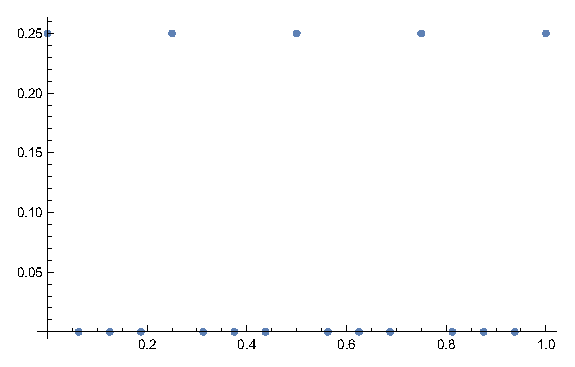
\includegraphics{img/Shor_gr1.eps}

\begin{doublespace}
\noindent\(\pmb{\text{(*Procesar medidas para tener la factorizaci{\' o}n*)}}\\
\pmb{\text{(*Fracciones continuas*)}}\\
\pmb{\text{L1}=\text{Table}[\{\text{Denominator}[\text{FromContinuedFraction}[\text{ContinuedFraction}[\text{Transpose}[L][[2,i]]]]],L[[i,3]]\},\{i,1,16\}];}\\
\pmb{\text{For}[i=1,i\leq \text{Dimensions}[\text{L1}][[1]],i\text{++},\text{For}[j=1,j\leq \text{Dimensions}[\text{L1}][[1]],j\text{++},\text{If}[\text{L1}[[i,1]]==\text{L1}[[j,1]]\&\&i\neq
j,\text{L1}[[i,2]]\text{+=}\text{L1}[[j,2]];}\\
\pmb{\text{L1}=\text{Drop}[\text{L1},\{j\}];]]]}\\
\pmb{\text{For}[i=1,i\leq \text{Dimensions}[\text{L1}][[1]],i\text{++},\text{If}[\text{OddQ}[\text{L1}[[i,1]]],\text{L1}=\text{Drop}[\text{L1},\{i\}];]]}\\
\pmb{\text{For}\left[i=1,i\leq \text{Dimensions}[\text{L1}][[1]],i\text{++},\text{If}\left[\text{Mod}\left[x^{\text{L1}[[i,1]]},M\right]\neq 1,\text{L1}=\text{Drop}[\text{L1},\{i\}];\right]\right]}\\
\pmb{\text{For}\left[i=1,i\leq \text{Dimensions}[\text{L1}][[1]],i\text{++},\text{If}\left[\text{GCD}\left[x^{\frac{\text{L1}[[1,1]]}{2}},M\right]==M-1,\text{L1}=\text{Drop}[\text{L1},\{i\}];\right]\right]}\\
\pmb{\text{For}\left[i=1,i\leq \text{Dimensions}[\text{L1}][[1]],i\text{++},\text{L1}[[i,2]]=\frac{\text{L1}[[i,2]]}{\text{Sum}[\text{L1}[[j,2]],\{j,1,\text{Dimensions}[\text{L1}][[1]]\}]};\right]}\\
\pmb{\text{L2}=\text{Table}\left[\left\{\text{GCD}\left[x^{\frac{\text{L1}[[i,1]]}{2}}+1,M\right],\text{L1}[[i,2]]\right\},\{i,1,\text{Dimensions}[\text{L1}][[1]]\}\right];}\\
\pmb{\text{L3}=\text{Table}\left[\left\{\text{GCD}\left[x^{\frac{\text{L1}[[i,1]]}{2}}-1,M\right],\text{L1}[[i,2]]\right\},\{i,1,\text{Dimensions}[\text{L1}][[1]]\}\right];}\)
\end{doublespace}

\begin{doublespace}
\noindent\(\pmb{\text{(*Graficar probabilidad de cada posible orden estimado*)}}\\
\pmb{\text{L1}}\\
\pmb{\text{ListPlot}[\text{L1}]}\)
\end{doublespace}

\begin{doublespace}
\noindent\(\{\{16,\text{5.200010849845537$\grave{ }$*${}^{\wedge}$-33}+0. i\},\{8,\text{6.162975822039155$\grave{ }$*${}^{\wedge}$-33}+0. i\},\{4,1.\,
+0. i\}\}\)
\end{doublespace}

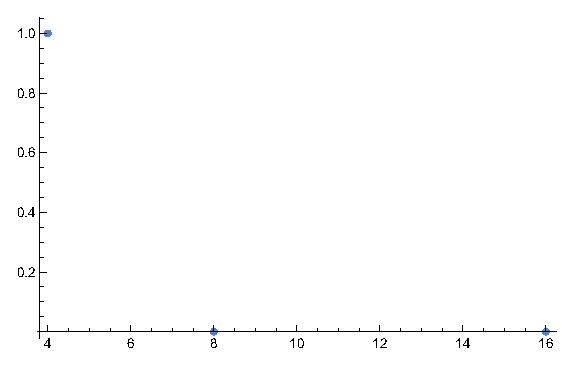
\includegraphics{img/Shor_gr2.eps}

\begin{doublespace}
\noindent\(\pmb{\text{(*Graficar la probabilidad de cada posible factorizaci{\' o}n hallada*)}}\\
\pmb{\text{L2}}\\
\pmb{\text{ListPlot}[\text{L2}]}\\
\pmb{\text{L3}}\\
\pmb{\text{ListPlot}[\text{L3}]}\)
\end{doublespace}

\begin{doublespace}
\noindent\(\{\{1,\text{5.200010849845537$\grave{ }$*${}^{\wedge}$-33}+0. i\},\{1,\text{6.162975822039155$\grave{ }$*${}^{\wedge}$-33}+0. i\},\{5,1.\,
+0. i\}\}\)
\end{doublespace}

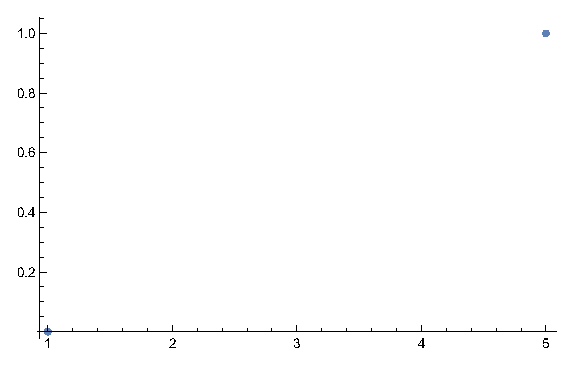
\includegraphics{img/Shor_gr3.eps}

\begin{doublespace}
\noindent\(\{\{15,\text{5.200010849845537$\grave{ }$*${}^{\wedge}$-33}+0. i\},\{15,\text{6.162975822039155$\grave{ }$*${}^{\wedge}$-33}+0. i\},\{3,1.\,
+0. i\}\}\)
\end{doublespace}

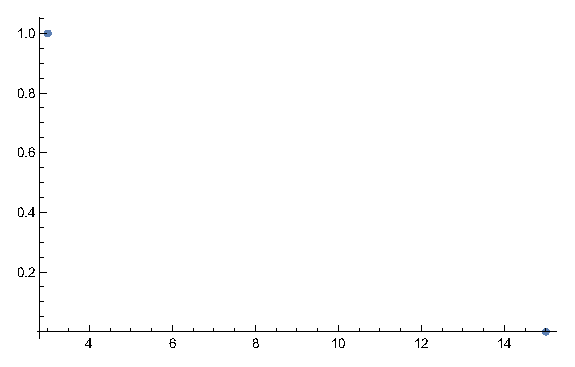
\includegraphics{img/Shor_gr4.eps}


\section{Simulación en Python}


\begin{verbatim}
import matplotlib.pyplot as plt
import matplotlib as mpl
import numpy as np
from scipy.stats import norm
from qutip import *
import tgates8
import time


#Transformada inversa de Fourier
def QFT4d(psi0, target1, target2, target3, target4):
    res = tgates8.SWAP(psi0, target2, target3)
    res = tgates8.SWAP(res.states[-1], target1, target4)
    res = tgates8.H(res.states[-1], target4)
    res = tgates8.CP(res.states[-1], target4, target3, -2*np.pi/2**2)
    res = tgates8.H(res.states[-1], target3)
    res = tgates8.CP(res.states[-1], target4, target2, -2*np.pi/2**3)
    res = tgates8.CP(res.states[-1], target3, target2, -2*np.pi/2**2)
    res = tgates8.H(res.states[-1], target2)
    res = tgates8.CP(res.states[-1], target4, target1, -2*np.pi/2**4)
    res = tgates8.CP(res.states[-1], target3, target1, -2*np.pi/2**3)
    res = tgates8.CP(res.states[-1], target2, target1, -2*np.pi/2**2)
    return tgates8.H(res.states[-1], target1)

#Compuerta de SWAP controlada
def CSWAP(psi0, control, target1, target2):
    res = tgates8.CCNOT(psi0, control, target1, target2)
    res = tgates8.CCNOT(psi0, control, target2, target1)
    return tgates8.CCNOT(psi0, control, target1, target2)

#Operador de multiplicación por 7 módulo 15 controlado
def CMUL7(psi0, control, target1, target2, target3, target4):
    res = tgates8.CNOT(psi0, control, target1)
    res = tgates8.CNOT(res.states[-1], control, target2)
    res = tgates8.CNOT(res.states[-1], control, target3)
    res = tgates8.CNOT(res.states[-1], control, target4)
    res = CSWAP(res.states[-1], control, target2, target3)
    res = CSWAP(res.states[-1], control, target1, target2)
    return CSWAP(res.states[-1], control, target1, target4)

#Dimensión del espacio de Hilbert
qN = 2**8


# El algoritmo
# Estado fiducial
psi0 = tensor(basis(2,0), basis(2,0), basis(2,0), basis(2,0),
              basis(2,0), basis(2,0), basis(2,0), basis(2,0))

# Preparación del estado inicial
res = tgates8.X(psi0, 7)

qsave(res, 'rp_0')

# Transformada de Hadamard en el primer registro
res = tgates8.H(res.states[-1], 0)
res = tgates8.H(res.states[-1], 1)
res = tgates8.H(res.states[-1], 2)
res = tgates8.H(res.states[-1], 3)

qsave(res, 'rp_1')

# Aplicando CMUL7(c=3)^1
res = CMUL7(res.states[-1], 3, 4, 5, 6, 7)

qsave(res, 'rp_2')

# Aplicando CMUL7(c=2)^2
res = CMUL7(res.states[-1], 2, 4, 5, 6, 7)
res = CMUL7(res.states[-1], 2, 4, 5, 6, 7)

qsave(res, 'rp_3')

# Aplicando CMUL7(c=1)^4
res = CMUL7(res.states[-1], 1, 4, 5, 6, 7)
res = CMUL7(res.states[-1], 1, 4, 5, 6, 7)
res = CMUL7(res.states[-1], 1, 4, 5, 6, 7)
res = CMUL7(res.states[-1], 1, 4, 5, 6, 7)

qsave(res, 'rp_4')

# Aplicando CMUL7(c=0)^8
res = CMUL7(res.states[-1], 0, 4, 5, 6, 7)
res = CMUL7(res.states[-1], 0, 4, 5, 6, 7)
res = CMUL7(res.states[-1], 0, 4, 5, 6, 7)
res = CMUL7(res.states[-1], 0, 4, 5, 6, 7)
res = CMUL7(res.states[-1], 0, 4, 5, 6, 7)
res = CMUL7(res.states[-1], 0, 4, 5, 6, 7)
res = CMUL7(res.states[-1], 0, 4, 5, 6, 7)
res = CMUL7(res.states[-1], 0, 4, 5, 6, 7)

qsave(res, 'rp_5')

# Aplicando la transformada cuántica inversa de Fourier sobre el primer registro
res = QFT4d(res.states[-1], 0, 1, 2, 3)

qsave(res, 'rp_6')

\end{verbatim}

\begin{figure}[H]
\centering 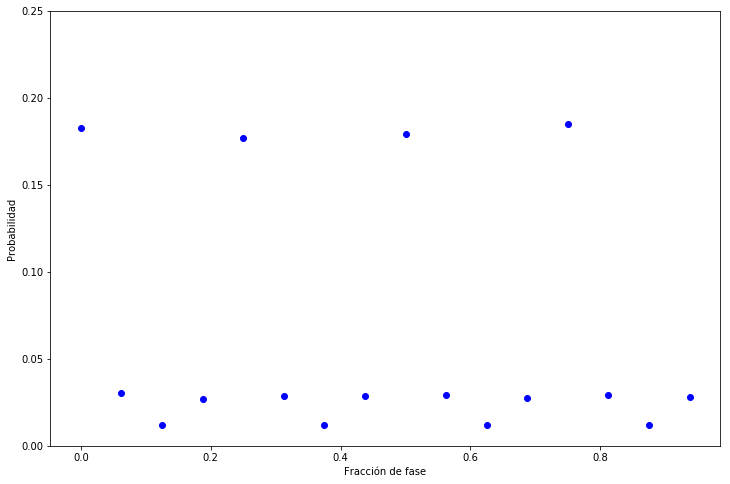
\includegraphics[width=0.9\linewidth]{img/shorlossless.png}
\caption{}
\end{figure}

[0.18265120316248348,
 0.030148605498127055,
 0.0117556126084082,
 0.027068348030583445,
 0.17700021614033762,
 0.028491802773181096,
 0.011881438650927171,
 0.028510782606300467,
 0.17917422966710292,
 0.029450553218688075,
 0.012081135256705483,
 0.027710388875941253,
 0.18489803932544116,
 0.02936951642045106,
 0.012035158723792341,
 0.027772969041529337]

